\documentclass[a4paper,12pt, headsepline, ngerman]{scrartcl}

%%%%%%%%%%%%%%%%%%%%%%% PACKAGES %%%%%%%%%%%%%%%%%%%%%%%%%%%%%%%%%%%%%%%%%%%%%%%%
\usepackage{scrlayer-scrpage}
\usepackage[nodisplayskipstretch]{setspace}     %vspace before/after math mode
\usepackage{geometry}
\usepackage{listings}                           %\lstinline[language=C]!while{$a || $b}!
\usepackage{babel}				                %Silbentrennung mit ngerman
\usepackage{booktabs} 			                % For prettier tables
\usepackage{mathtools}  		                %Mathe-Paket
\usepackage{color}				                %\textcolor{blue}{text...}
\usepackage[dvipsnames]{xcolor}                 %Mehr Auswahl bei Farben
\usepackage[T1]{fontenc}		                %Umlaute
\usepackage[utf8]{inputenc}
\usepackage{wrapfig}
\usepackage{caption}
\usepackage{ulem}                               %Durchstreichen von Wörtern mit \sout{text}
\usepackage{adjustbox}
\usepackage{enumitem}				            %Aufzählungen [label=\alph*)]
\usepackage{tcolorbox} 				            %Merkboxen
\usepackage{marvosym}                           %\Lightning
\usepackage{multirow}
\usepackage[hidelinks]{hyperref}			    %Hyperlinks setzen
\usepackage[answerdelayed]{exercise}	        %Nach hyperref einbinden!
%%%%%%%%%%%%%% FARBEN %%%%%%%%%%%%%%%%%%%%%%%%%%%%%%%%%%%%%%%%%%%%%%%%%%%%%%%%%%%%%%
\definecolor{codegreen}{rgb}{0,0.6,0}
\definecolor{codegray}{rgb}{0.5,0.5,0.5}
\definecolor{codepurple}{rgb}{0.58,0,0.82}
\definecolor{codeback}{rgb}{0.95,0.95,0.92}
\definecolor{codebasic}{rgb}{0,0,0.8}
\definecolor{codekeyword}{rgb}{0.8,0,0}
\definecolor{tcback}{rgb}{.95,.95,.95}          %tcolorbox Hintergrund
\definecolor{tcframe}{rgb}{.89,.15,.21}         %tcolorbox Umrandung
%%%%%%%%%%%%%%% KONFIGURATION VON PACKAGES %%%%%%%%%%%%%%%%%%%%%%%%%%%%%%%%%%%%%%%%%%%%
\geometry{a4paper, portrait, left=1.5cm, right=2cm, top=1cm, bottom=2cm, headsep=0.2cm, includehead, head=27.30193pt}
\setlist[enumerate]{nosep, topsep=0pt}	        %Kleinere Abstände bei Aufzählungen
\setlist[itemize]{noitemsep, topsep=0pt}
\lstdefinestyle{mystyle}{
	language=HTML,
    basicstyle=\color{codebasic}\ttfamily,
	backgroundcolor=\color{codeback},
	commentstyle=\color{codegreen},
	keywordstyle=\color{codekeyword},
    tagstyle=\color{codekeyword},
	numberstyle=\tiny\color{codegray},
	stringstyle=\color{codepurple},
	breakatwhitespace=false,
	breaklines=true,
	captionpos=b,
	keepspaces=false,
	extendedchars=true,
	numbers=none,
	numbersep=5pt,
	showspaces=false,
	showstringspaces=false,
	showtabs=false,
	tabsize=2,
	columns=fullflexible %erzeugt keine komischen Leerzeichen mehr, die man erst beim Kopieren sieht
}
\lstset{style=mystyle}
\lstset{literate=%
	{Ö}{{\"O}}1
	{Ä}{{\"A}}1
	{Ü}{{\"U}}1
	{ß}{{\ss}}1
	{ü}{{\"u}}1
	{ä}{{\"a}}1
	{ö}{{\"o}}1
	{~}{{\textasciitilde}}1
}
\setkomafont{headsepline}{\color{black}}
%Exercise-Paket Umbenennungen
\renewcommand{\listexercisename}{Liste der Aufgaben}%
\renewcommand{\ExerciseName}{Aufgabe}%
\renewcommand{\AnswerName}{L{\"o}sung zu Aufgabe}%
\renewcommand{\ExerciseListName}{Aufg.}%
\renewcommand{\AnswerListName}{L{\"o}sung}%
\renewcommand{\ExePartName}{Teil}%
\renewcommand{\ArticleOf}{von\ }%
\renewcommand{\ExerciseHeader}{%
	\textbf{\large\ExerciseHeaderDifficulty\ExerciseName\ %
	\ExerciseHeaderNB\normalsize\ExerciseHeaderTitle\ExerciseHeaderOrigin}\medskip}
\renewcommand{\AnswerHeader}{
	\medskip\textbf{L{\"o}sung zu \ExerciseName\ \ExerciseHeaderNB}\smallskip}
%tcolorbox Konfiguration
\tcbset{
%	frame code={}
%	center title,
%	left=0pt,
%	right=0pt,
%	top=0pt,
%	bottom=0pt,
	fonttitle=\large\bfseries,
	colback=tcback,
	colframe=tcframe,
%	width=\dimexpr\textwidth\relax,
%	enlarge left by=0mm,
%	boxsep=5pt,
%	arc=0pt,outer arc=0pt,
}
%%%%%%%%%%%%%%%%%%%%%% STYLE %%%%%%%%%%%%%%%%%%%%%%%%%%%%%%%%%%%
\pagestyle{headings} %KOMA-Script mit Kopf-Fuß-Zeilen
\raggedbottom
\raggedright
\onehalfspacing
\def\pics{./pics}

\begin{document}
	\setlength\parindent{0pt} %keine Einrückungen beim Start eines Paragraphen

	%Header
	\lohead{HTML}
	%\cohead{} %im Arbeitsblatt
	\rohead{}
	\cofoot[\pagemark]{\pagemark}
	\title{HTML

	Ein Skript für das Berufskolleg}
	\author{Hermann Maier}
	\maketitle
	\thispagestyle{empty}
	\newpage
	\null\vfill
	\copyright \the\year{} Maier, Hermann, \href{mailto:maier@privatemail.com}{maier@privatemail.com}

    \begin{tcolorbox}\raggedright
        Aktuelle Version inklusive Quelldateien unter \href{https://github.com/hoerm007/HTMLSkript_KaufmBK_BW}{https://github.com/hoerm007/HTMLSkript\_KaufmBK\_BW}
    \end{tcolorbox}

	Dieses Werk unterliegt der CC BY-NC-SA 4.0 Lizenz \href{https://creativecommons.org/licenses/by-nc-sa/4.0/legalcode.de}{https://creativecommons.org/licenses/by-nc-sa/4.0/legalcode.de}.

	Sie dürfen:
	\begin{itemize}
		\item Teilen — das Material in jedwedem Format oder Medium vervielfältigen und weiterverbreiten
		\item Bearbeiten — das Material remixen, verändern und darauf aufbauen
	\end{itemize}
	Unter folgenden Bedingungen:
	\begin{itemize}
		\item Namensnennung - Sie müssen angemessene Urheber- und Rechteangaben machen , einen Link zur Lizenz beifügen und angeben, ob Änderungen vorgenommen wurden. Diese Angaben dürfen in jeder angemessenen Art und Weise gemacht werden, allerdings nicht so, dass der Eindruck entsteht, der Lizenzgeber unterstütze gerade Sie oder Ihre Nutzung besonders.
		\item Nicht kommerziell - Sie dürfen das Material nicht für kommerzielle Zwecke nutzen.
		\item Weitergabe unter gleichen Bedingungen - Wenn Sie das Material remixen, verändern oder anderweitig direkt darauf aufbauen, dürfen Sie Ihre Beiträge nur unter derselben Lizenz wie das Original verbreiten.
	\end{itemize}
	\newpage
	\tableofcontents
	\thispagestyle{empty}
	\newpage
	\def\pics{./pics}
	\rohead{}
	% !TeX root = ../Skript_HTML.tex
\cohead{\Large\textbf{Begriffe und Grundgerüst}}
\section{Begriffe und Grundgerüst}
Das Internet ist aus unserer heutigen Welt nicht mehr wegzudenken. Im WWW findet man Informationen jeder Art, man kauft ein, trifft sich und kommuniziert rund um den ganzen Globus.  Das WWW unter Eingabe der URL zu nutzen, ist heute selbstverständlich geworden. Eine Webseite jedoch mit HTML zu erstellen, welche von einem Browser angezeigt werden kann, beherrschen nur wenige. Um die Grundlagen von HTML Schritt für Schritt zu erlernen, werden wir eine eigene Webseite erstellen. Wir beschränken uns auf die Grundlagen, d.h. wir werden einen einfachen Texteditor zum Erstellen verwenden anstatt einer Entwicklungsumgebung. Zum Anzeigen der Webseite werden wir einen normalen Browser wie Chrome, Firefox oder Edge verwenden.

Eine Webseite ist letztendlich eine Datei. Standardmäßig ist diese Datei in der Auszeichnungssprache HTML erstellt. Wir werden also selbst eine solche Datei erstellen. Greift man mit Hilfe eines Browsers über das Internet auf eine Seite zu, so wird diese HTML-Datei über das Internet an den eigenen PC übertragen und dann vom Browser interpretiert und dargestellt. Eine HTML-Datei kann man aber auch einfach auf dem eigenen PC erstellen, bearbeiten und betrachten.

\begin{Exercise}[title=Für was steht die Abkürzung HTML und was versteht man unter dem Begriff einer Auszeichnungssprache? Die Begriffe maschinenlesbare Sprache und Tag sind hier besonders wichtig., label=Auszeichnungssprache]
\end{Exercise}

Wir erstellen Schritt für Schritt unsere eigene Webseite.

\begin{Exercise}[title=Erstelle deine erste Webseite., label=DateiErstellen]

    Erstelle in deinem Heimverzeichnis (Laufwerk mit deinem Anmeldenamen) einen Ordner \textit{HTML}. Öffne den Editor und kopiere folgenden Text:

    \begin{lstlisting}
<html>

<head>

<title>Schülerseite</title>

</head>

<body>

Willkommen auf meiner Webseite!

<br>

<br>

<p>Ich bin Schüler des WG West in Stuttgart.</p>

</body>

</html>
    \end{lstlisting}
    Speichere die Datei nun als \textit{schueler.html} in deinem HTML-Ordner. (Datei\(\rightarrow\)speichern unter\(\rightarrow\)Dateityp auf Alle Dateien ändern.)
    Diese Datei kann nun mit einem Browser geöffnet werden.
\end{Exercise}

\begin{Exercise}[title=Recherchiere die Funktion der oben verwendeten Tags., label=Tags]

    Tipp: Die Webseite \href{https://www.w3schools.com/tags/default.asp}{w3schools.com} verfügt über eine Übersicht aller Tags.
\end{Exercise}


	\newpage
    % !TeX root = ../Skript_HTML.tex
\cohead{\Large\textbf{Sonderzeichen}}
\section{Umlaute und Sonderzeichen}
Je nach Betriebssystem und Browser kann es zu Problemen bei der Darstellung von Zeichen kommen, insbesondere bei Umlauten:

\begin{minipage}[t]{0.8\textwidth}
    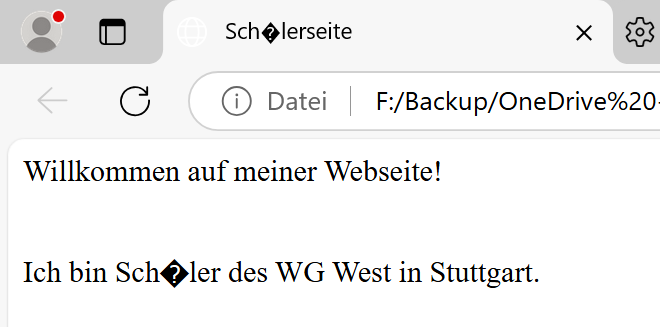
\includegraphics[width=\linewidth]{\pics/Umlaute.png}
\end{minipage}

Um solche Probleme zu vermeiden, ist es empfehlenswert, die Umlaute durch bestimmte Zeichenfolgen, sogenannte Escape-Sequenzen, zu ersetzen, z.B. statt ä im Quellcode \lstinline|\&auml;| zu schreiben. Im Internet lassen sich verschiedenen Listen mit diesen Zeichenfolgen finden.

\begin{Exercise}[title=, label=Umlaute]
    \begin{enumerate}
        \item Füge zwischen den head-Tags (\lstinline|<head> ... </head>|) den folgenden Tag ein: \lstinline|<meta charset="utf-8">|
        \item Schaue dir dann deine Seite nochmals im Browser an.
        \item Ersetze alle Umlaute durch Escape-Sequenzen und verwende in Zukunft diese statt den Umlauten oder dem scharfen s.
        \item Prüfe nochmals im Browser, ob die Umlaute nun alle korrekt dargestellt werden.
        \item Ändere nun noch die Codierung deiner Datei auf UTF-8. Gehe dazu im Editor nochmals auf Speichern unter\(\rightarrow\)Dateityp auf alle Dateien ändern und Codierung auf UTF-8. (Hinweis: Oft wird die Datei standardmäßig bereits mit UTF-8 gespeichert.)
    \end{enumerate}
    \begin{minipage}[t]{\textwidth}
        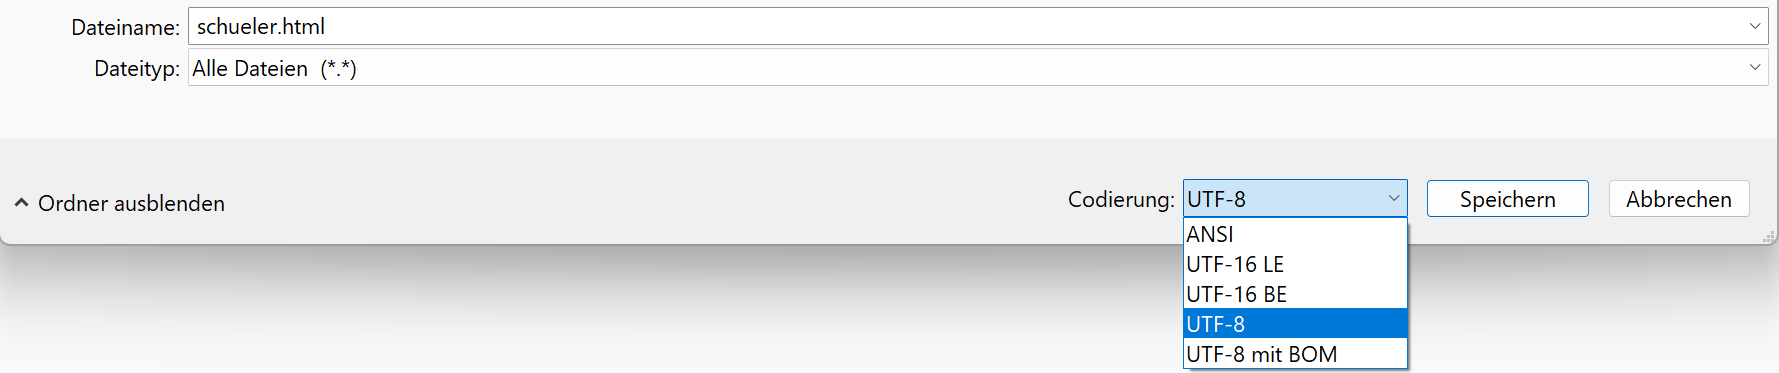
\includegraphics[width=\linewidth]{\pics/UTF8Speichern.png}
    \end{minipage}%
\end{Exercise}
    \newpage
    % !TeX root = ../Skript_HTML.tex
\cohead{\Large\textbf{Validieren}}
\section{Validieren}
HTML existiert seit Ende der 80er und hat sich mit der Zeit stark verändert. Zum Beispiel gibt es Unmengen an Tags, die als deprecated, d.h. veraltet markiert sind. Diese Tags sollten eigentlich nicht mehr verwendet werden aber es stehen noch viele Webseiten online, die diese Tags verwenden. Die best practices, also das empfohlene Vorgehen beim Erstellen von Webseiten hat sich ebenfalls stark gewandelt. Bis heute haben Browser unterschiedliche Funktionsumfänge, z.B. ist das Format JPG für Bilder veraltet. Es gibt deutlich bessere Formate, die aber jeweils nicht von allen Browsern unterstützt werden.

Lange Rede, kurzer Sinn, HTML ist ein Sammelsurium verschiedenster Techniken, um Webseiten zu gestalten, von denen viele aus Gründen der Abwärtskompatibilität noch unterstützt werden aber nicht mehr verwendet werden sollen. Wie kann Ottonormalschüler entscheiden, ob er seine Webseite vernünftig erstellt hat? Die empfohlenen Techniken werden regelmäßig (alle paar Jahre) in einem Standard zusammengefasst, aktuell HTML 5.2. Nur, weil ein Browser eine Webseite korrekt darstellt, muss die Webseite noch lange nicht dem Standard entsprechen. Glücklicherweise gibt es Validatoren, die prüfen, ob eine Webseite dem Standard entspricht.

\begin{Exercise}[title=Prüfe deine Webseite (schueler.html in deinem Heimverzeichnis) mit einem Validator, label=Validator1]

    Zum Beispiel W3Schools stellt unter  von \href{https://validator.w3.org/#validate_by_upload}{validator.w3.org} einen Validator zur Verfügung.
\end{Exercise}

\bigskip

Unsere Webseite entspricht also nicht dem Standard, wird aber von einem Browser (vermutlich) korrekt dargestellt.

\begin{Exercise}[title=Passe deine Webseite so an{,} dass sie dem Standard entspricht., label=Validator2]
    Ergänze am Anfang deiner Webseite noch vor dem \lstinline|<html>|-Tag folgenden Tag: \lstinline|<!DOCTYPE html>|.
    Erweitere den \lstinline|<html>|-Tag zu  \lstinline|<html  lang="de">|

    Informiere dich über die Bedeutung der eingefügten Tags und validiere deine Webseite dann nochmals.
\end{Exercise}
    \newpage
    % !TeX root = ../Skript_HTML.tex
\cohead{\Large\textbf{Textauszeichnungen}}
\section{Textauszeichnungen}
Auf Webseiten können Teile von Texten ausgezeichnet werden, um sie hervorzuheben. Hierbei wird zwischen physischen und logischen Auszeichnungen unterschieden. Bei den physischen Auszeichnungen handelt es sich lediglich um optische Auszeichnungen, so dass Texte z.B. Fett oder Kursiv dargestellt werden. Eine besondere Bedeutung haben physisch ausgezeichnete Texte jedoch nicht. Bei logisch ausgezeichneten Texten, z.B. Überschriften oder Zitaten, ist das jedoch anders. Wenn man Texte logisch auszeichnet, dann erhalten die Texte auch eine entsprechende Bedeutung.

Ein Beispiel sind die beiden Tags \lstinline|<i>...</i>| und \lstinline|<em>...</em>|. Beide Tags stellen den Text in der Regel kursiv dar. Das \lstinline|<i>|-Tag steht für italic (deutsch kursiv). Es ist eine physische/optische Auszeichnung. Das \lstinline|<em>|-Tag steht für emphasize (deutsch hervorheben/betonen) und ist eine logische Auszeichnung, die in der Regel vom Browser ebenfalls als kursiver Text dargestellt wird. Wenn beide Tags zu kursivem Text führen, wo ist der Unterschied? Der Unterschied liegt im Wesentlichen darin, wie der Computer den Text auffasst:

Die beiden Sätze \lstinline|HTML ist <i>super</i> und toll| und \lstinline|HTML ist <em>super</em> und toll| werden im Browser zwar gleich angezeigt. Würde man jedoch eine KI fragen was HTML ist, so würde sie beim ersten Satz sagen, dass HTML super und toll ist und beim zweiten Satz, dass HTML insbesondere super ist und außerdem auch toll.

Seit HTML 5 sollen Texte auf Webseiten nur gemäß ihrer Bedeutung logisch ausgezeichnet werden. Das ist aus verschiedenen Gründen wichtig. Dazu zählen unter anderem:
\begin{itemize}
    \item Barrierefreiheit: Sehbehinderte bzw. blinde Menschen können die Texte auf Webseiten z.B. mit Screenreader lesen. Wenn Texte logisch ausgezeichnet werden, dann hilft das dabei, den Aufbau, die Struktur und die Inhalte der Webseite besser zu verstehen. Wenn man z.B. bei einem normalen Absatz lediglich die Schriftgröße so einstellt, dass es aussieht wie eine Überschrift, jedoch nicht als Überschrift auszeichnet, dann könnte man bei der Betrachtung am Bildschirm zwar annehmen, dass der Text eine Überschrift darstellen soll. Blinde Menschen können das jedoch nicht und für sie ist der Text ein ganz normaler Absatz. Daher ist es für sie eine große Hilfe, wenn man Texte gemäß ihrer Bestimmung auszeichnet.
    \item Auslesen durch Suchmaschinen: Die Aufnahme in die Suchmaschinen erfolgt in der Regel durch sogenannte Bots. Das sind Programme, die selbständig im Internet Webseiten auslesen und in den Suchmaschinenindex aufnehmen. Um die Struktur und die Inhalte einer Webseite zu erkennen und zu gewissen Suchbegriffen einzuordnen, wird unter anderem die Seite inkl. aller Texte und logischer Auszeichnungen ausgewertet. Kommt ein Begriff z.B. in einer Überschrift vor, so ist die Wahrscheinlichkeit, dass die Webseite interessante Infos zu diesem Begriff enthält größer, als wenn der Begriff nur im Fließtext vorkommt.
    \item Auslesen durch andere Programme: Was für Suchmaschinen gilt, das gilt auch für andere Programme wie z.B. LLMs/KIs, die Webseiten auslesen. Wenn z.B. in sozialen Netzwerken eine Webseite geteilt wird, wird häufig die Überschrift sowie ein Ausschnitt aus dem Text und evtl. ein Bild als Vorschau angezeigt. Wenn die Texte nicht entsprechend ausgezeichnet wurden (z.B. die Überschrift als Überschrift deklariert im Unterschied zu einfach die Schriftgröße vergrößert), dann werden solche Vorgänge erschwert.
    \item Aufbau einer Suchfunktion: Viele Webseiten nehmen nach einer gewissen Zeit sehr große Ausmaße an, sodass eine Suchfunktion auf der Webseite notwendig wird. Auch hierbei ist man darauf angewiesen, dass die Texte gemäß ihrer Bestimmung logisch ausgezeichnet werden. So kann man diesen eine gewisse Gewichtung verleihen. Wenn z.B. ein Suchbegriff auf verschiedenen Seiten in der Überschrift und in den Absätzen vorkommt, dann könnte man den Suchalgorithmus so programmieren, dass die Seite, die den Begriff in der Überschrift enthält eine höhere Gewichtung erhält. Man könnte die Suche auch so eingrenzen, sodass z.B. nur in den Überschriften gesucht wird.
\end{itemize}
\begin{Exercise}[title=Füge deiner Webseite Textauszeichnungen hinzu., label=Textauszeichnungen]

    Die Textelemente der Webseite sollen nun wie im Bild gezeigt ausgezeichnet werden. Zudem soll der spätere Betrachter wissen, um wessen Website es sich dabei handelt. Daher soll eine Überschrift eingefügt werden.
    \begin{minipage}[t]{\textwidth}
        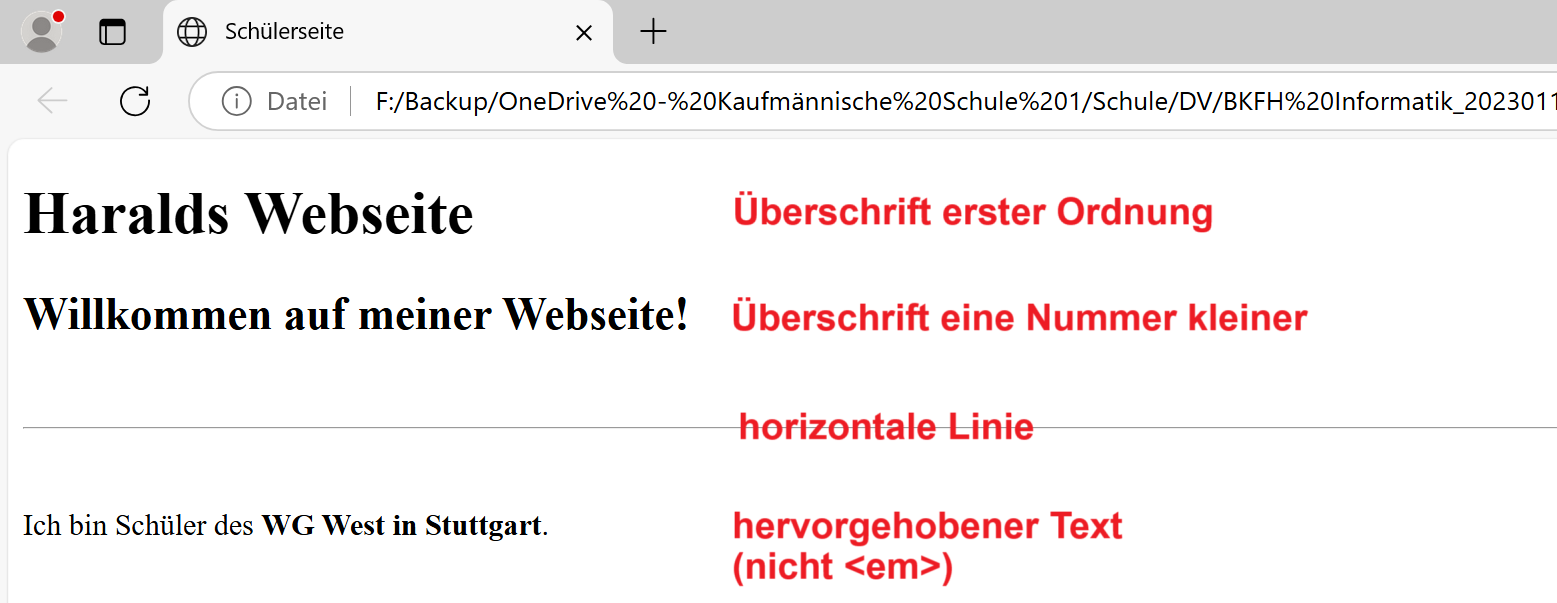
\includegraphics[width=\linewidth]{\pics/Textauszeichnungen.png}
    \end{minipage}
    Erweitere deine Datei \textit{schueler.html} mit dem Windows-Editor entsprechend der Vorgaben im Bild. Recherchiere dabei die notwendigen Tags.

    Validiere dann deine Datei \textit{schueler.html}.
\end{Exercise}



    \newpage
    % !TeX root = ../Skript_HTML.tex
\cohead{\Large\textbf{CSS}}
\section{Cascading Style Sheets}
Es gibt zwar noch immer HTML-Tags, die zur Formatierung der Webseite dienen, wie z.B. Ändern der Schriftfarbe, jedoch sind so gut wie alle diese Tags als veraltet (deprecated) markiert. Veraltete Tags werden zwar noch unterstützt, sollten aber nicht mehr verwendet werden. In ferner Zukunft werden Browser diese Tags nicht mehr unterstützen wodurch es dann zu Darstellungsfehlern im Browser kommen wird.

Der grundlegende Style (Formatierung abgesehen von physischen Textauszeichnungen) wird über das sogenannte CSS festgelegt. CSS steht für Cascading Style Sheets, was zusätzliche Dateien impliziert. Dies ist jedoch nicht immer notwendig. CSS lässt sich auf 3 möglichen Wegen verwenden:
\begin{enumerate}
    \item Inline, indem man ein style-Attribut innerhalb eines HTML-Tags verwendet, falls man tatsächlich nur die Formatierung dieses einen Tags ändern will, z.B. wird \lstinline|<strong style="color:red;">Beispieltext</strong>| hervorgehoben und Rot dargestellt.
    \item Intern innerhalb einer Datei, indem man ein \lstinline|<style>|-Tag in den \lstinline|<head>|-Bereich der HTML-Datei einfügt, falls man die Formatierung innerhalb dieser einen Datei ändern will. Diese Einträge sind mit denen, die wir in einer CSS-Datei anlegen werden identisch, nur, dass sie in die HTML-Datei geschrieben werden.
    \item Extern, indem man über ein  \lstinline|<link>|-Tag im \lstinline|<head>|-Bereich der HTML-Datei eine externe CSS-Datei einbindet. Diese Datei kann man in verschiedenen HTML-Dateien einbinden und so die Formatierung für mehrere Webseiten zentral verwalten.
\end{enumerate}

Wir werden nur die externe Variante verwenden. Die anderen Varianten sind von der Verwendung her gleich nur der Ort, an dem man die Formatierungsanweisungen angibt, ändert sich.

\begin{Exercise}[title=, label=CSS1]
    \begin{enumerate}
        \item Erzeuge mit dem Editor eine leere Datei und speichere diese unter \textit{style.css} im selben Ordner wie \textit{schueler.html}. Auf die Dateiendung achten! Nicht als \textit{style.css.txt} speichern.
        \item Binde die CSS-Datei in die Schülerseite im  \lstinline|<head>|-Bereich von \textit{schueler.html} ein:
        \lstinline|<link href="style.css" rel="stylesheet" type="text/css">|
    \end{enumerate}
\end{Exercise}
In der CSS-Datei kann man nun für verschiedene Tags die Formatierung ändern. Die Syntax einer CSS-Datei dazu sieht wie folgt aus:

\lstinline|Tagname (mehrere kommaseparierte Tags zulässig){Eigenschaft:neuer Wert;}|

Will man z.B. die Farbe der größten Überschriften in Blau ändern, so fügt man folgenden Eintrag hinzu: \lstinline|h1 {color:blue;}|

Man kann in den geschweiften Klammern beliebig viele Eigenschaften ändern. Die Namen und zulässigen Werte können z.B. bei w3schools gefunden werden.

\begin{Exercise}[title=, label=CSS2]
    Nimm (über die CSS-Datei) folgende Änderungen für die bisherige Seite vor:
    \begin{enumerate}
        \item Die Hintergrundfarbe soll auf gelb gesetzt werden (informiere dich in diesem Zusammenhang über die Farbangabe mit Hilfe des RGB-Codes).
        \item Alle Überschriften sollen immer Rot und unterstrichen dargestellt werden.
        \item Die Überschriften ersten Grades sollen immer zentriert ausgegeben werden.
    \end{enumerate}
    Validiere dann deine Datei \textit{schueler.html}.
\end{Exercise}


    \newpage
    % !TeX root = ../Skript_HTML.tex
\cohead{\Large\textbf{Listen}}
\section{Listen}
Damit man etwas mehr über den Webseitenersteller erfährt, soll die Webseite um zwei Listen nach folgendem Muster erweitert werden:
wissen, um wessen Website es sich dabei handelt. Daher soll eine Überschrift eingefügt werden.
\begin{minipage}[t]{\textwidth}
    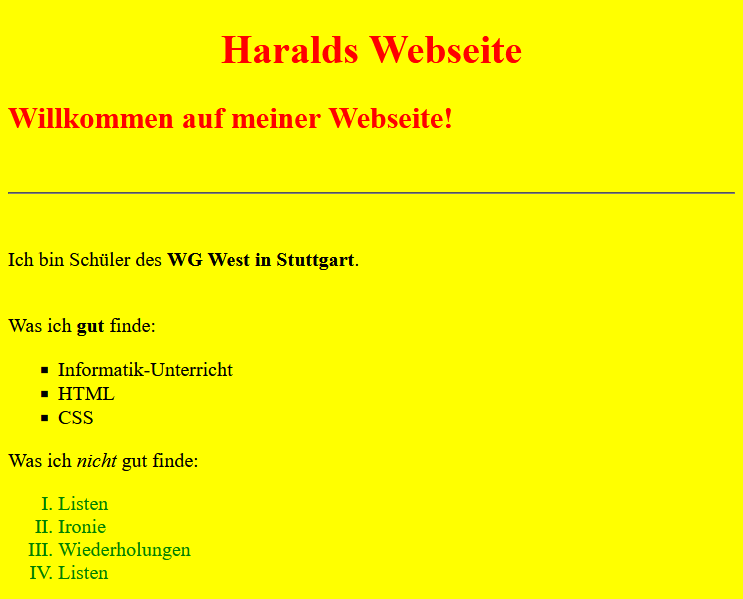
\includegraphics[width=\linewidth]{\pics/Listen.png}
\end{minipage}

\begin{Exercise}[title=, label=Listen]
    \begin{enumerate}
        \item Erweitere deine \textit{schueler.html} mit dem Windows-Editor entsprechend des obigen Bildes. Recherchiere dazu die Tags für Listen (geordnete und ungeordnete Listen).
        \item Validiere dann deine Datei \textit{schueler.html}.
        \item Nimm über die CSS-Datei folgende Änderungen vor (wie auch im Screenshot zu sehen):
        \begin{itemize}
            \item Der Aufzählungstyp für ungeordnete Listen soll nun quadratisch sein.
            \item Der Aufzählungstyp für geordnete Listen sollen nun große römische Ziffern sein und die geordneten Listen sollen in Grün dargestellt werden.
        \end{itemize}
    \end{enumerate}
\end{Exercise}


    \newpage
    % !TeX root = ../Skript_HTML.tex
\cohead{\Large\textbf{Bilder}}
\section{Bilder}
Eine Webseite lebt von Bildern. Um die Webseite optisch ansprechender zu machen, wird ein Bild eingefügt (Das Bild wurde mittels \href{https://www.canva.com/}{canva.com} KI-erzeugt):
\begin{minipage}[t]{\textwidth}
    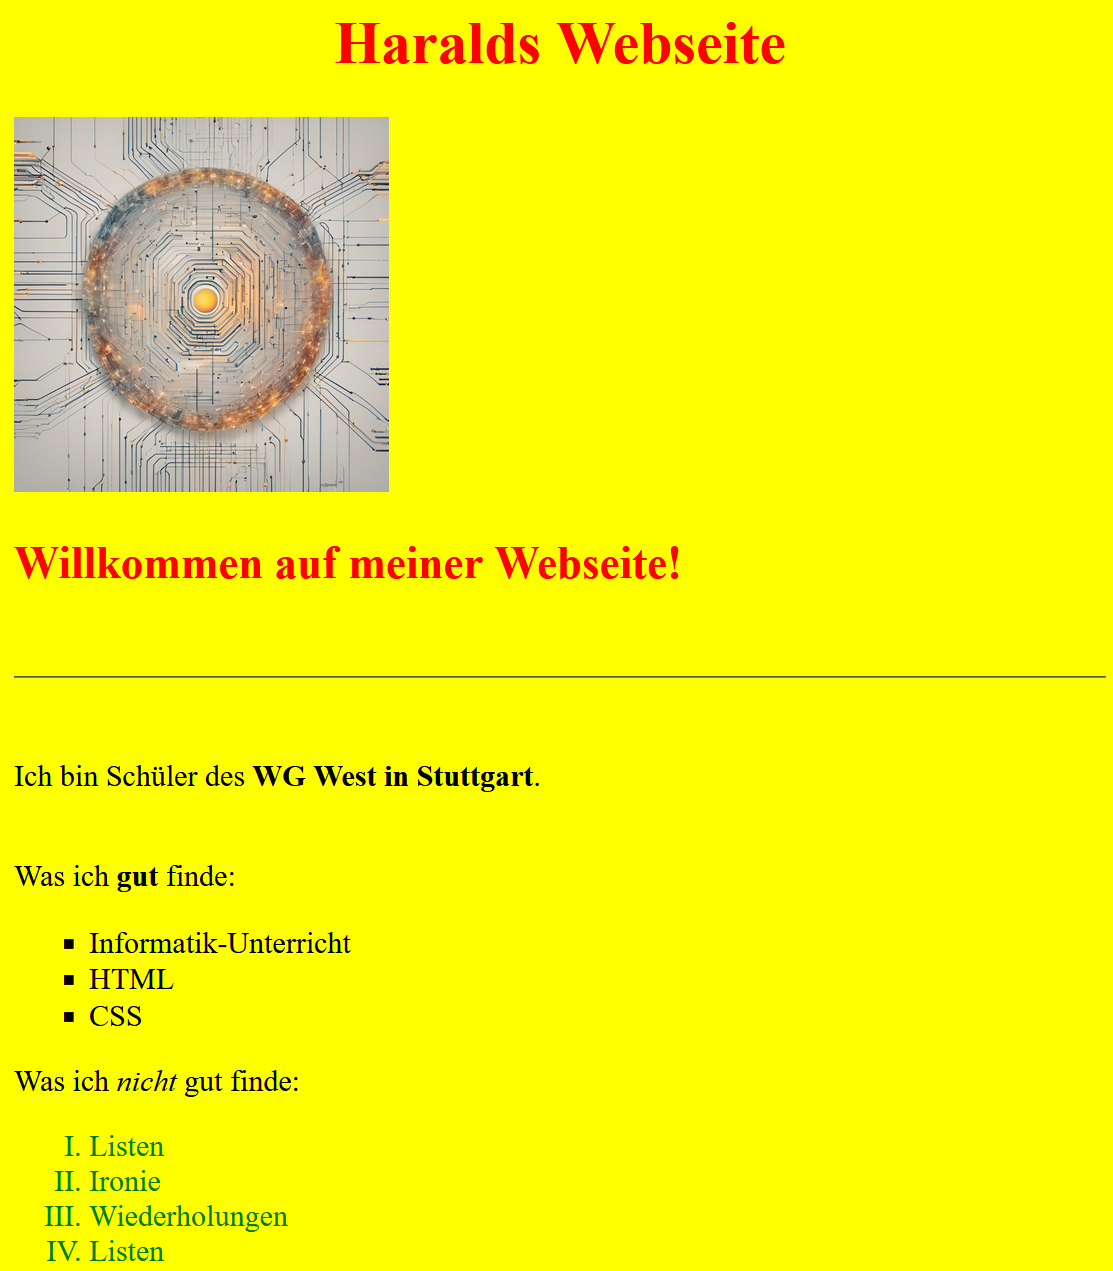
\includegraphics[width=\linewidth]{\pics/BilderEinfuegen.png}
\end{minipage}
\begin{Exercise}[title=, label=Bilder]
    \begin{enumerate}
        \item Lade dir ein Bild aus dem Internet herunter und speichere dieses in einem Ordner Bilder, der im gleichen Verzeichnis wie \textit{schueler.html} liegt. Kurze Dateinamen machen das Einbinden leichter.
        \item Binde in deiner \textit{schueler.html} das Bild ein. Recherchiere dazu den Tag für das Einfügen von Bildern. Erkundige dich, welche Attribute für die Höhen- und Breitenangabe von Bildern notwendig sind und was der Alternativtext bei Bildern bedeutet.
        \item Um ein Bild einzubinden, muss man einen Dateipfad angeben. Wie funktionieren relative und absolute Pfadangaben? Welche Vor- und Nachteile bieten die beiden Möglichkeiten?
    \end{enumerate}
    Informiere dich über die wesentlichen Bildformate (Rasterbilder wie jpg, gif, png oder Vektorgrafiken wie svg) und deren Unterschiede. Wichtige Begriffe sind hier unter anderem Dateigröße, Komprimierung, Transparenz, Farbraum.
\end{Exercise}



    \newpage
    % !TeX root = ../Skript_HTML.tex
\cohead{\Large\textbf{Abschnitte}}
\section{Abschnitte definieren und formatieren}
Häufig will man einen ganzen Abschnitt einer Webseite gleich formatieren, z.B. wollen wir den oberen Teil der Webseite komplett zentrieren:
\begin{minipage}[t]{\textwidth}
    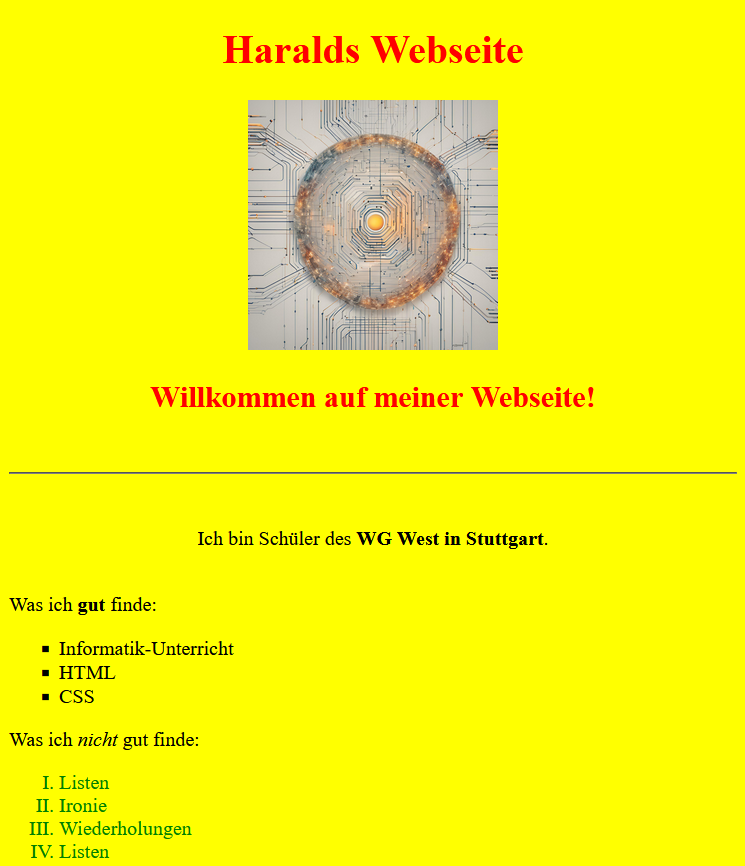
\includegraphics[width=\linewidth]{\pics/Abschnitte.png}
\end{minipage}
Dazu bietet HTML das \lstinline|<div>...</div>|-Tag an. Dabei steht div für division bzw. Abschnitt auf Deutsch. Das Tag kann man um einen beliebig großen Teil des bodys der Webseite schreiben. Man kann beliebig viele solcher Abschnitte definieren und jeden solchen Abschnitt dann formatieren. Dazu erstellen wir in der CSS-Datei eine eigene Klasse.

Bisher haben wir in der CSS-Datei Eintragungen vom Typ \lstinline|tagname {attributName1:Wert; attributName2:Wert;}|. Der Syntax für eigene Klassen ist dem für Tags ganz ähnlich. Wir beginnen nun nur mit einem Punkt statt dem Namen des Tags: \lstinline|.klassenName {attributName1:Wert, attributName2:Wert;}|.

\begin{Exercise}[title=, label=Abschnitte]
    \begin{enumerate}
        \item Erstelle eine eigene Klasse mit beliebigem Namen in deiner CSS-Datei mit dem Attribut \lstinline|text-align| und dem Wert \lstinline|center|.
        \item Ändere dein \textit{schueler.html} so ab, dass der obere Teil bis einschließlich \textit{WG West in Stuttgart} zentriert ist. Recherchiere dazu wie man ein \lstinline|<div>|-Tag mit einer eigenen CSS-Klasse verwendet.
    \end{enumerate}
\end{Exercise}
    \newpage
    % !TeX root = ../Skript_HTML.tex
\cohead{\Large\textbf{Links}}
\section{Verlinkungen}
Die Vernetzung von Inhalten über so genannte Links ist ein wesentliches Merkmal des WWW. Aber auch eine normale Homepage besteht in der Regel bereits aus mehreren Seiten, die mit einander verlinkt sind. Man kann aber auch auf die Seiten anderer Anbieter eine Verlinkung setzen.
\begin{minipage}[t]{\textwidth}
    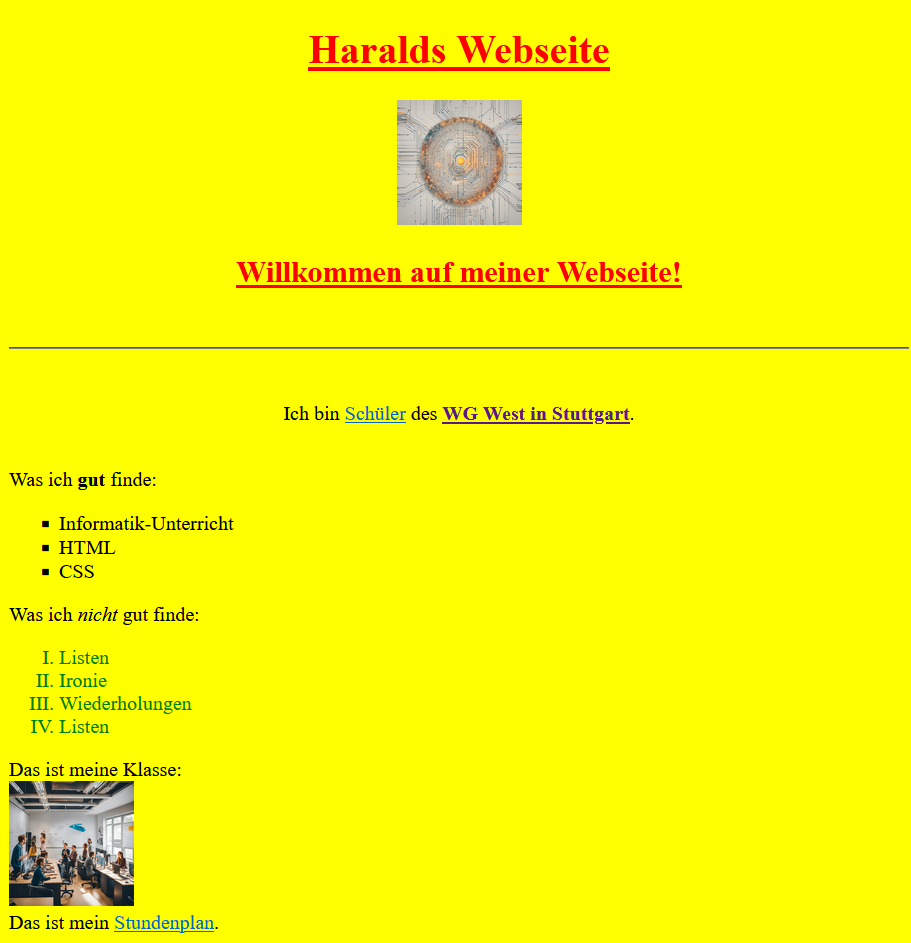
\includegraphics[width=\linewidth]{\pics/Links.png}
\end{minipage}
\begin{Exercise}[title=, label=Links]
    \begin{enumerate}
        \item Erstelle eine Datei \textit{stundenplan.html} im gleichen Ordner wie \textit{schueler.html} mit folgendem Inhalt:
        \begin{lstlisting}
            <!DOCTYPE html>
            <html lang="de">
            <head>
            <link href="style.css" rel="stylesheet" type="text/css">
            <title>Unterricht</title>
            <meta charset="utf-8">
            </head>
            <body>
            So sieht mein Stundenplan aus:
            </body>
            </html>
        \end{lstlisting}
        \item Ergänze deine Webseite wie im Bild zu sehen (du kannst ein beliebiges Bild einbinden. Das Beispielbild wurde mittels \href{https://www.canva.com/}{canva.com} KI-erzeugt). Hinweis: Die beiden Bilder wurden verkleinert, damit das Beispielbild nicht zu groß wird.
        Für das zweite Bild kannst du wieder ein beliebiges Bild aus dem Internet verwenden. Stelle eine Höhe von 400 Pixeln ein.
        \item Erstelle einen Link von WG West in Stuttgart auf die Homepage des WG Wests (\text{https://www.wg-west.de/}).
        \item Erstelle einen Link von Stundenplan auf \textit{stundenplan.html}.
        \item Je nach Größe der eingefügten Bilder ist die Webseite inzwischen so groß, dass nun Scrollen nach unten notwendig ist. Um direkt auf das Bild der Klasse (und weitere Informationen) zu kommen, soll eine Verknüpfung von Schüler direkt auf das Bild führen. Informiere dich über diese Art der Verknüpfung innerhalb einer Datei auf eine ID.
        \item Validiere dann deine Datei \textit{schueler.html}.
    \end{enumerate}
\end{Exercise}
    \newpage
    % !TeX root = ../Skript_HTML.tex
\cohead{\Large\textbf{Tabellen}}
\section{Tabellen}
Bei der Gestaltung einer Website sollte immer die Übersichtlichkeit im Vordergrund stehen. Um Inhalte, Schrift oder Bilder strukturiert darstellen zu können, benötigt man häufig Tabellen. Mit Hilfe einer Tabelle kann man z.B. den Stundenplan übersichtlich darstellen.

\begin{Exercise}[title=Erstelle deinen Stundenplan in \textit{stundenplan.html}, label=Tabellen1]
    \begin{enumerate}
        \item Informiere dich über Tabellen. Beachte dabei den Unterschied zwischen Tabellenüberschriften und normalen Tabellendaten.
        \item Erstelle einen Beispielstundenplan (Bsp. siehe Bilder weiter unten).
        \item Verbinde alle Zellen der letzten Spalte und füge eine Verlinkung zu \textit{schueler.html} ein.
    \end{enumerate}
\end{Exercise}
Deine Webseite sollte dann ungefähr so aussehen:

\begin{minipage}[t]{\textwidth}
    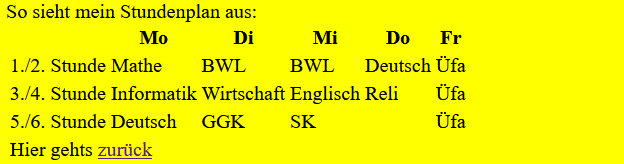
\includegraphics[width=0.8\linewidth]{\pics/TabelleOhneFormatierung.png}
\end{minipage}%

\begin{Exercise}[title=Formatiere deine Tabelle mit Hilfe von CSS, label=Tabellen2]
    \begin{enumerate}
        \item Der Inhalt der Tabelle soll zentriert sein.
        \item Die Tabelle und die einzelnen Zellen sollen schwarze Gitternetzlinien bekommen.
        \item Die Tabellenüberschriften sollen kursiv sein.
        \item Die Tabellenüberschriften und -inhalte sollen blau sein.
        \item Die Tabelle soll zentriert und 800px breit sein.
        \item Validiere dann deine Datei \textit{stundenplan.html}.
    \end{enumerate}
\end{Exercise}

\begin{minipage}[t]{\textwidth}
    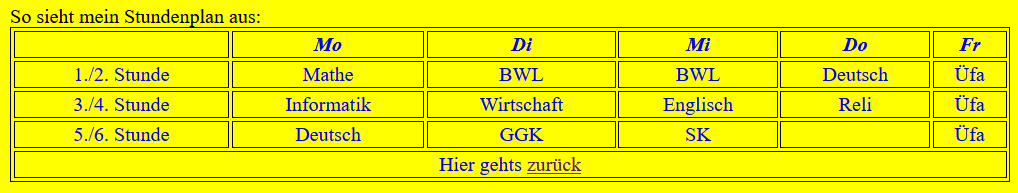
\includegraphics[width=\linewidth]{\pics/TabelleMitFormatierung.png}
\end{minipage}%
    \newpage
    \input{./Arbeitsblaetter/Lösungen.tex}
\end{document}

